\documentclass{article}
\iffalse
This file is protected by Copyright. Please refer to the COPYRIGHT file
distributed with this source distribution.

This file is part of OpenCPI <http://www.opencpi.org>

OpenCPI is free software: you can redistribute it and/or modify it under the
terms of the GNU Lesser General Public License as published by the Free Software
Foundation, either version 3 of the License, or (at your option) any later
version.

OpenCPI is distributed in the hope that it will be useful, but WITHOUT ANY
WARRANTY; without even the implied warranty of MERCHANTABILITY or FITNESS FOR A
PARTICULAR PURPOSE. See the GNU Lesser General Public License for more details.

You should have received a copy of the GNU Lesser General Public License along
with this program. If not, see <http://www.gnu.org/licenses/>.
\fi

\usepackage{listings} % for coding language styles
\usepackage{fancyhdr}
\usepackage{colortbl}
\usepackage{tabularx}
\newcolumntype{C}{>{\centering\arraybackslash}X}
\usepackage[margin=.75in]{geometry}
\pagestyle{fancy}
\lhead{Application Worker Data Sheet}
\rhead{ANGRYVIPER Team}
\renewcommand{\headrulewidth}{0pt}
\usepackage{array}
\newcolumntype{P}[1]{>{\centering\arraybackslash}p{#1}}
\newcolumntype{M}[1]{>{\centering\arraybackslash}m{#1}}
\usepackage{graphicx}
\graphicspath{ {figures/} }
\usepackage{amsmath}
\usepackage{pdflscape}
\usepackage[justification=centering]{caption}
\usepackage{subcaption}
\usepackage{hyperref}
\usepackage{tikz}
\setlength\parindent{0pt}
\definecolor{blue}{rgb}{.7,.8,.9}
\definecolor{drkgreen}{rgb}{0,.6,0}
\usetikzlibrary{arrows, decorations.markings, positioning, backgrounds}
% for double arrows http://www.texample.net/tikz/examples/double-arrows/
\tikzstyle{vecArrow} = [thick, decoration={markings,mark=at position
   1 with {\arrow[semithick]{open triangle 60}}},
   double distance=1.4pt, shorten >= 5.5pt,
   preaction = {decorate},
   postaction = {draw,line width=1.4pt, white,shorten >= 4.5pt}]
\tikzstyle{innerWhite} = [semithick, white,line width=1.4pt, shorten >= 4.5pt]
\newenvironment{absolutelynopagebreak}
  {\par\nobreak\vfil\penalty0\vfilneg
   \vtop\bgroup}
  {\par\xdef\tpd{\the\prevdepth}\egroup
   \prevdepth=\tpd}

\begin{document}

\section*{Summary - Time Demux}
	\begin{tabular}{|c|M{13.5cm}|}
		\hline
		\rowcolor{blue}
		• & • \\
		\hline
		Name & time\_demux \\
		\hline
		Version & 1.3.0 \\
		\hline
		Release Date & Feb 2018 \\
		\hline
		Component Library & training.components \\
		\hline
		Verification Model & None \\
		\hline
		Implementations & RCC \\
		\hline
		Tested Platforms & linux-zynq-arm, c7-x86\_64 \\
		\hline
	\end{tabular}

\section*{Functionality}
The Time Demux component acts as a demultiplexer/router by parsing an \verb+iqstream_with_sync+ protocol and routing timestamps and data to separate output ports.\\
\break
The incoming \verb+iqstream_with_sync+ supports three opcodes: \verb+iq+, \verb+Sync+, and \verb+Time+. The output ports use the \verb+iqstream+ and \verb+iqstream_with_sync+ protocols, the former using a single opcode. Data within the \verb+iqstream_with_sync+'s \verb+Time+ opcode (a single 64-bit value) is passed directly through, while data within the \verb+iq+ opcode is converted to \verb+iqstream+'s \verb+iq+ opcode's data (which, conveniently, is the same structure). The \verb+iqstream_with_sync+'s \verb+Sync+ opcode is currently ignored.\\

\section*{Block Diagrams}
	\subsection*{Top level}
\begin{center}
	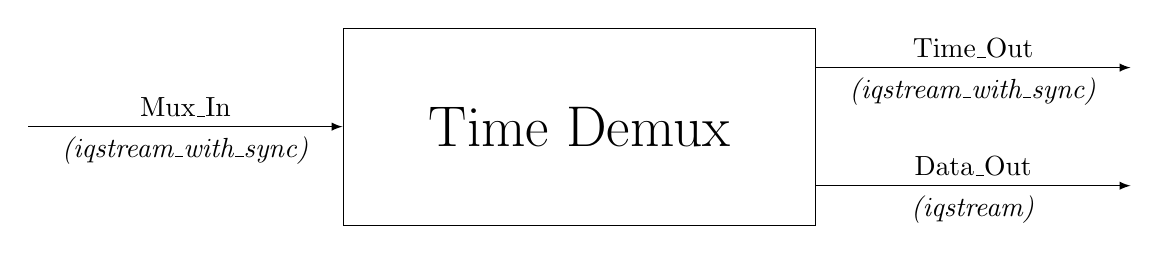
\begin{tikzpicture}
	\tikzstyle{sharp} = [-latex]
	\node (mytd) [draw,rectangle,minimum width=6cm,minimum height=2.5cm] {\huge Time Demux};
	\draw[sharp] (-7,0) -- node[midway, below]{\textit{(iqstream\_with\_sync)}} node[midway, above]{Mux\_In} (mytd);
	\draw[sharp] (3,0.75) -- node[midway, below]{\textit{(iqstream\_with\_sync)}} node[midway, above]{Time\_Out} (7,0.75);
	\draw[sharp] (3,-0.75) -- node[midway, below]{\textit{(iqstream)}} node[midway, above]{Data\_Out} (7,-0.75);
	\end{tikzpicture}
    \captionof{figure}{Top-level Block Diagram}
    \label{fig:block_diagram}
\end{center}

\section*{RCC source dependency}
	\begin{itemize}
		\item training/components/time\_demux.rcc/time\_demux.cc
	\end{itemize}

\begin{landscape}
\section*{Properties}
	\scriptsize
	\begin{tabular}{|c|c|c|c|c|c|c|c|c|c|}
		\hline
		\rowcolor{blue}
		Name & OCS & OWD RCC & OWD HDL & Type & Length & Accessibility & Valid Range & Default & Usage \\
		\hline
		Current\_Second & Property & N/A & N/A & ULong & N/A & Volatile & Default & N/A & Last seen ``second'' timestamp \\
		\hline
		Messages\_Read & Property & N/A & N/A & ULongLong & N/A & Volatile & Default & N/A & Number of messages seen \\
		\hline
		Bytes\_Read & Property & N/A & N/A & ULongLong & N/A & Volatile & Default & N/A & Total number of bytes read \\
		\hline
	\end{tabular}
\section*{Ports}
	\subsection*{Input / Consumer}
		\scriptsize
		\begin{tabular}{|c|c|c|M{10.2cm}|}
			\hline
			\rowcolor{blue}
			Port Name & Protocol & Optional & Notes \\
			\hline
			Mux\_In
			& iqstream\_with\_sync\_protocol
			& False
			& Time-stamped 16-bit I/Q data samples (32 bits per sample); \verb+Sync+ opcode ignored\\
			\hline
		\end{tabular}
	\subsection*{Output / Producer}
		\scriptsize
		\begin{tabular}{|c|c|c|c|M{10.2cm}|}
			\hline
			\rowcolor{blue}
			Port Name & Protocol & Optional & Notes \\
			\hline
			Time\_Out
			& iqstream\_with\_sync\_protocol
			& False
			& Only uses 64-bit timestamp in \verb+Time+ opcode; \verb+iq+ and \verb+Sync+ opcodes guaranteed not to be present\\
			\hline
			Data\_Out
			& iqstream\_protocol
			& False
			& 16-bit I/Q data samples (32 bits per sample) \\
			\hline
		\end{tabular}
\end{landscape}

\section*{Control Timing and Signals}
	N/A; this is an RCC-only component.

\section*{Performance and Resource Utilization}
	\subsubsection*{HDL}
	N/A; this is an RCC-only component.

	\subsubsection*{RCC}
	TBD.\\

	\begin{tabular}{|c|c|c|}
		\hline
		\rowcolor{blue}
		Processor Type & Processor Frequency & Run Function Time \\
		\hline
		linux-c6-x86\_64 Intel(R) Xeon(R) CPU E5-1607 & 3.00 GHz & TBD \\
		\hline
		linux-c7-x86\_64 Intel(R) Core(TM) i7-3630QM & 2.40 GHz & TBD \\
		\hline
		linux-zynq-arm ARMv7 Processor rev 0 (v7l) & 666 MHz & TBD \\
		\hline
	\end{tabular}

\normalsize
\section*{Test and Verification}

This component uses the standard OpenCPI test process. It is one of the few that use multiple ports. \textbf{}
\begin{center}
\framebox{\parbox{0.8\linewidth}{\centering The only currently known issue is that the specfile must define the ``Data\_Out'' port \textit{first} to have the test application use it to signal ``done.''}}
\end{center}

% AV-2921
\iffalse
\subsubsection*{Usage (local/x86)}
After building the worker, the user only needs to type \verb+make tests+ in the \textit{time\_demux.test} directory. Options can be added to the command line as noted above, e.g. \verb+make tests INFILE=mybigfile+.

\subsubsection*{Usage (remote/ARM)}
To test the worker on a remote system, the user must ensure the remote is mounting the local filesystem properly. That setup is outside the scope of this document.\medskip

By changing ``\verb+make tests+'' to ``\verb+make show+'' in the \textit{time\_demux.test} directory, the user will be instructed concerning how to test, e.g.:
\begin{verbatim}
Locally: rm -f odata/output_{time,data}.bin
On device: ocpirun -d -v -t -5 app_time_demux
Locally: make verify
\end{verbatim}
\medskip
\fi
\subsection*{Advanced / Detailed Theory of Operation}
\textbf{This section is not essential to understand to perform the training lab.}\\

Testing of the Time Demux component consists of a C++ program (\textit{test\_data\_generator.cxx}) used to generate input data and expected ``golden'' outputs (Figure \ref{fig:generator}).\medskip

Fake timestamps and sample data are interleaved into an input file using the ``message mode'' format required to have \textit{ocpi.file\_read} playback opcodes with data. The C++ generator takes input arguments of: input file name, starting timestamp, number of samples to push each ``second,'' filename for the interleaved file, filename for the golden timestamps, and filename for the golden output file. These parameters are all handled by the OpenCPI test XML, with the test application shown in Figure \ref{fig:test_application}.\medskip
\iffalse
There is one OAS or Application XML (\textit{app\_time\_demux.xml}) that connects standard CDK-provided file reader and file writers to the UUT
\fi

Output data is compared to the golden file(s) by the Makefile (Figure \ref{fig:test_setup}).

\begin{center}
\begin{absolutelynopagebreak}
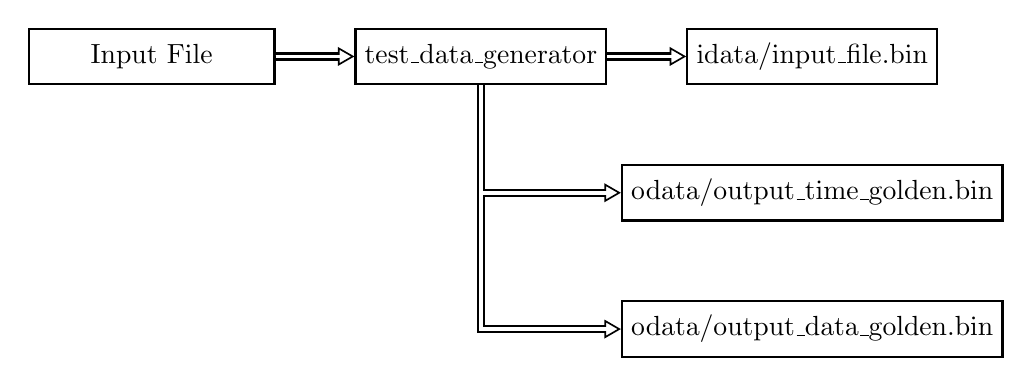
\begin{tikzpicture}[
  thick,
  minimum width={width("File Writer (data)")+10pt},
  minimum height={20pt},
  ]
  \node[draw,rectangle] (if) {Input File};
  \node[draw,rectangle,right = of if] (cxx) {test\_data\_generator};
  \node[draw,rectangle,right = of cxx] (inf) {idata/input\_file.bin};
  \node[draw,rectangle,fill=white,below = of inf] (gt) {odata/output\_time\_golden.bin};
  \node[draw,rectangle,fill=white,below = of gt] (gd) {odata/output\_data\_golden.bin};
  \draw[vecArrow] (if) to (cxx);
  \draw[vecArrow] (cxx) to (inf);
  \draw[vecArrow] (cxx) |- (gt);
  \draw[vecArrow] (cxx) |- (gd);
  % Fix broken corner:
  \draw[innerWhite] (cxx) |- (gt);
  \draw[innerWhite] (cxx) |- (gd);
\end{tikzpicture}
\captionof{figure}{C++ Generator Usage}
\label{fig:generator}
\end{absolutelynopagebreak}
\bigskip

\begin{absolutelynopagebreak}
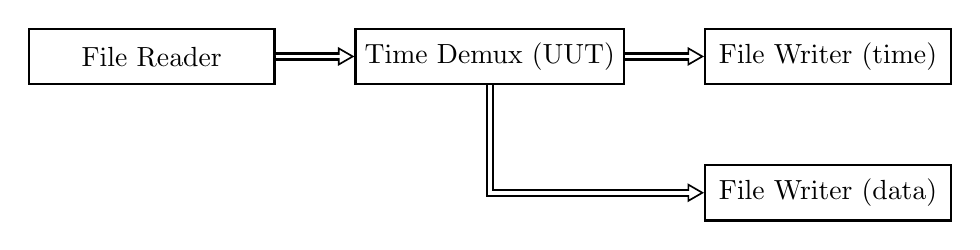
\begin{tikzpicture}[
  thick,
  minimum width={width("File Writer (data)")+10pt},
  minimum height={20pt},
  ]
  \node[draw,rectangle] (fr) {File Reader};
  \node[draw,rectangle,right = of fr] (td) {Time Demux (UUT)};
  \node[draw,rectangle,fill=white,right = of td] (tfw) {File Writer (time)};
  \node[draw,rectangle,fill=white,below = of tfw] (dfw) {File Writer (data)};
  \draw[vecArrow] (fr) to (td);
  \draw[vecArrow] (td) to (tfw);
  \draw[vecArrow] (td) |- (dfw);
\end{tikzpicture}
\captionof{figure}{Test Application Layout (\textit{app\_time\_demux})}
\label{fig:test_application}
\end{absolutelynopagebreak}
\bigskip

\begin{absolutelynopagebreak}
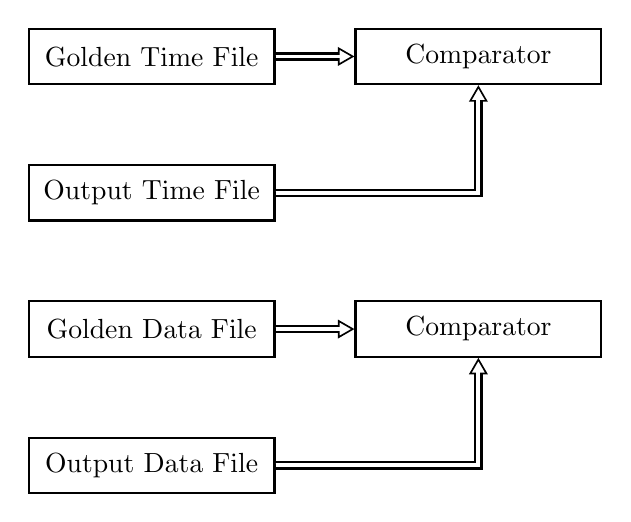
\begin{tikzpicture}[
  thick,
  minimum width={width("File Writer (data)")+10pt},
  minimum height={20pt},
  ]
  \node[draw,rectangle] (gt) {Golden Time File};
  \node[draw,rectangle,below = of gt] (uutt) {Output Time File};
  \node[draw,rectangle,below = of uutt] (gd) {Golden Data File};
  \node[draw,rectangle,below = of gd] (uutd) {Output Data File};
  \node[draw,rectangle,right = of gt] (comparet) {Comparator};
  \node[draw,rectangle,right = of gd] (compared) {Comparator};
  \draw[vecArrow] (gt) to (comparet);
  \draw[vecArrow] (uutt) -| (comparet);
  \draw[vecArrow] (gd) to (compared);
  \draw[vecArrow] (uutd) -| (compared);
  % Note to anybody copy/pasting: you need to draw "innerWhite"s
  % over any intersections without nodes.
\end{tikzpicture}
\captionof{figure}{Testing}
\label{fig:test_setup}
\end{absolutelynopagebreak}
\end{center}
\bigskip

The default XML provides reasonable values for each of the data generator's required parameters:\\
	\begin{tabularx}{\textwidth}{|c|C|C|}
		\hline
		\rowcolor{blue}
		Test Property & Default & Notes \\
		\hline
		IFILE & (Running kernel image) \textit{e.g.} \verb+/boot/vmlinuz-3.10.0-327.4.4.el7.x86_64+ & The input file is truncated to a 32-bit boundary to simulate two 16-bit data samples. This may cause verification issues if using random files.\\
		&  & \\
		\hline
		START & 0 & Decimal only \\
		\hline
		SAMPLES & 256 & Should not exceed 2048 \\
		\hline
	\end{tabularx}\\

\medskip
For test purposes, the ``timestamp'' is a one-up counter starting at START placed in the upper 32-bits and then incremented and placed into the lower 32-bits:

% [language=X]
\begin{lstlisting}
$ od -t x8 odata/output_time_golden.bin | head
0000000 0000000000000001 0000000100000002
0000020 0000000200000003 0000000300000004
0000040 0000000400000005 0000000500000006
0000060 0000000600000007 0000000700000008
0000100 0000000800000009 000000090000000a
0000120 0000000a0000000b 0000000b0000000c
0000140 0000000c0000000d 0000000d0000000e
0000160 0000000e0000000f 0000000f00000010
0000200 0000001000000011 0000001100000012
0000220 0000001200000013 0000001300000014
\end{lstlisting}
\medskip

By default, output golden data is written as \textit{INPUTFILE\_gold\_data} and \textit{INPUTFILE\_gold\_time} in the same path as \textit{INPUTFILE}. The \textit{INPUTFILE} named here is the interleaved file whose name is provided by the test framework and is the \textbf{output} of \textit{test\_data\_generator}, based on the IFILE Property.

\end{document}
